\section{Prompts}
\label{app:prompts}
We reproduce the instructions used for the DSPy signatures on the evaluation runs, without the input and output fields, and concatenating multi-line lists into sentences.

\begin{lstlisting}[title={LayerChildGenerationSignature (Phase 1, one layer of children)}]
Generate children for a specific parent node in the research DAG.
You are a research planning expert. Given a parent research question and the current DAG structure, generate focused sub-questions that can be answered independently to collectively answer the parent question. Look at the entire DAG context to ensure coherence and avoid duplication.
Guidelines:
1. Generate focused, standalone sub-questions that collectively answer the parent
2. Consider the existing DAG structure to maintain coherence
3. Respect the max_children limit strictly
4. Each child should be answerable independently
5. Output format should always be "list" (bullet points)
\end{lstlisting}

\begin{lstlisting}[title={CompositionInstructionSignature (Phase 1, per parent)}]
Write explicit parent composition instructions referencing each child node.
Given a parent node and its children, explain exactly how the child answers will be combined to produce the parent's output. Always reference children by their IDs so downstream steps can trace dependencies unambiguously.
\end{lstlisting}

\begin{lstlisting}[title={LeafNodeResearcher (Phase 2, leaves)}]
Answer a leaf node research task using literature search results.
Given literature search results and the expected output format, provide an answer that strictly adheres to the format requirements.
Format types and requirements:
- boolean: Provide "Yes." or "No." followed by a single sentence justification with citations.
- short_answer/list/report: Provide 3-5 bullet points ('- ' prefix) summarizing key takeaways with citations.
- table_csv/json: Provide structured data (CSV or JSON) with inline citations in headers or cells.
CRITICAL: Preserve all citations from the literature search in [X] format. Do not add citations that aren't in the source material.
\end{lstlisting}

\begin{lstlisting}[title={ParentNodeSynthesizer (Phase 2, parents)}]
Synthesize answers from child nodes to answer a parent node's research task.
Given the answers from all child subtasks and composition instructions, combine them to produce the answer for the parent task in the required format.
CRITICAL RULES:
1. Use ONLY the information from the child results - no external knowledge
2. Follow the composition instructions exactly
3. When citing evidence, use the citation numbers [1], [2], etc. from the AVAILABLE CITATIONS section - do NOT reference child nodes by name
4. Output in the specified format
5. If child results contradict, acknowledge and explain the contradiction
\end{lstlisting}

\begin{lstlisting}[title={GapExplorer (Phase 2, refinement, first pass)}]
Explore potential gaps that could enhance the composed answer.
This is the FIRST PASS - be creative and identify any areas where the answer could be improved, even if they're minor enhancements. Don't filter yet.
Think about: missing perspectives or viewpoints. Unaddressed sub-questions or aspects. Areas that could use more depth or detail. Counterarguments or alternative viewpoints not covered. Quantitative data or evidence gaps. Temporal or geographic coverage gaps. Edge cases or exceptions not mentioned.
Return a list of potential gaps, even if they seem minor. The second pass will determine which ones are critical enough to warrant refinement.
\end{lstlisting}

\begin{lstlisting}[title={GapImportanceEvaluator (Phase 2, refinement, second pass)}]
Evaluate whether identified gaps are important enough to warrant refinement.
This is the SECOND PASS - evaluate gaps based on the specified conservatism level.
CONSERVATISM MODES:
- "conservative": Only flag gaps that are CRITICAL - the answer would be misleading or fundamentally incomplete without this information. Default to NOT refining.
- "balanced": Flag gaps that would SIGNIFICANTLY improve the answer's completeness, depth, or accuracy. Be moderate - refine if the gap meaningfully enhances quality.
- "aggressive": Flag gaps that would improve the answer, even if moderately. Refine if the gap would add value, even if not critical.
Consider: Would adding this information fundamentally change the answer's conclusion? Is this gap misleading or would it cause the answer to be wrong? Would a reasonable reader say the answer is incomplete without this? Is this a core aspect of the question that's missing? How much would this gap improve the answer's quality?
Provide a confidence score (0.0-1.0) indicating how confident you are that refinement is warranted.
\end{lstlisting}

\begin{lstlisting}[title={OutlineFromDAGSignature (Phase 3)}]
Generate a report outline that structures a persuasive argument from DAG research.
The DAG represents a research question decomposed into sub-questions. Each node answered a question through research. The root node has the final answer. Child nodes contain supporting evidence that led to that answer.
Create an outline for a persuasive report arguing a definitive stance for the root answer. Use the DAG's hierarchy to organize evidence: child findings support parent conclusions. Structure as a logical argument (Executive Summary, Evidence Sections, Conclusion).
REQUIREMENTS: Start with Executive Summary stating root answer prominently. Organize body sections to build argument logically using DAG hierarchy. Use ## for main sections, ### for subsections. Design for prose writing (paragraphs, not just lists). Base outline ONLY on content actually present in root_answer (no placeholders).
\end{lstlisting}

\begin{lstlisting}[title={ReportFromDAGSignature (Phase 3)}]
Generate a comprehensive final report from the DAG results.
The report must: 1. Start with the root answer prominently (matching its format) 2. Follow the provided outline structure 3. Incorporate findings from all DAG nodes 4. Take a clear stance that matches the root answer 5. Preserve all citations [X] from the DAG 6. Be well-written, coherent, and comprehensive
CRITICAL STANCE ALIGNMENT: If root answer is "Yes" (boolean), the report must argue FOR that position. If root answer is "No" (boolean), the report must argue AGAINST. If root answer is a list, the report should be organized around those items. The report's conclusion must align with the root answer. Do not contradict or hedge against the root answer's stance.
FORMATTING REQUIREMENTS: The report title (# heading) should be the CLAIM, not the question. Use proper markdown. Write in prose paragraphs with supporting bullet points where appropriate. Do not include internal node references in the output. Only use citation numbers like [1], [2], [3]. Every section must contain substantive content from the dag_results. Do not include a bibliography section (it is added later).
\end{lstlisting}

\section{An Example DAG}
\label{app:dag}
\Cref{fig:dag} shows a DAG from a logged run that considered whether the US federal government should substantially increase social services for persons living in poverty. In this example run, we set the DAG depth to 2. The initial planner decomposed the question into the current landscape of federal services, and the likely effects of increasing services. Each of those two topics were further decomposed into 2 leaf questions. After the composition of the landscape node, the refinement check found that child care and family tax credit information was missing, so the pipeline attached a refinement subtree with 2 new leaves (shown shaded).

Across the \dagLeaves{} leaves of this run, we retrieved \dagLeafSources{} distinct sources (\dagLeafSourcesMean{} per leaf, on average). Of the \dagRootSources{} sources available at the root, \dagRootFromRefinement{} of them were from the refinement subtree. Thus, the refinement step contributed about a third of the total evidence base. The final report has \dagReportWords{} words, \dagReportCitations{} citations, and cites all \dagReportSources{} sources. \Cref{sec:citations} shows that the citations do not match the claims they support. We provide the full log in the repository, which shows the answers and citations of each node.

\begin{figure}[t]
\centering
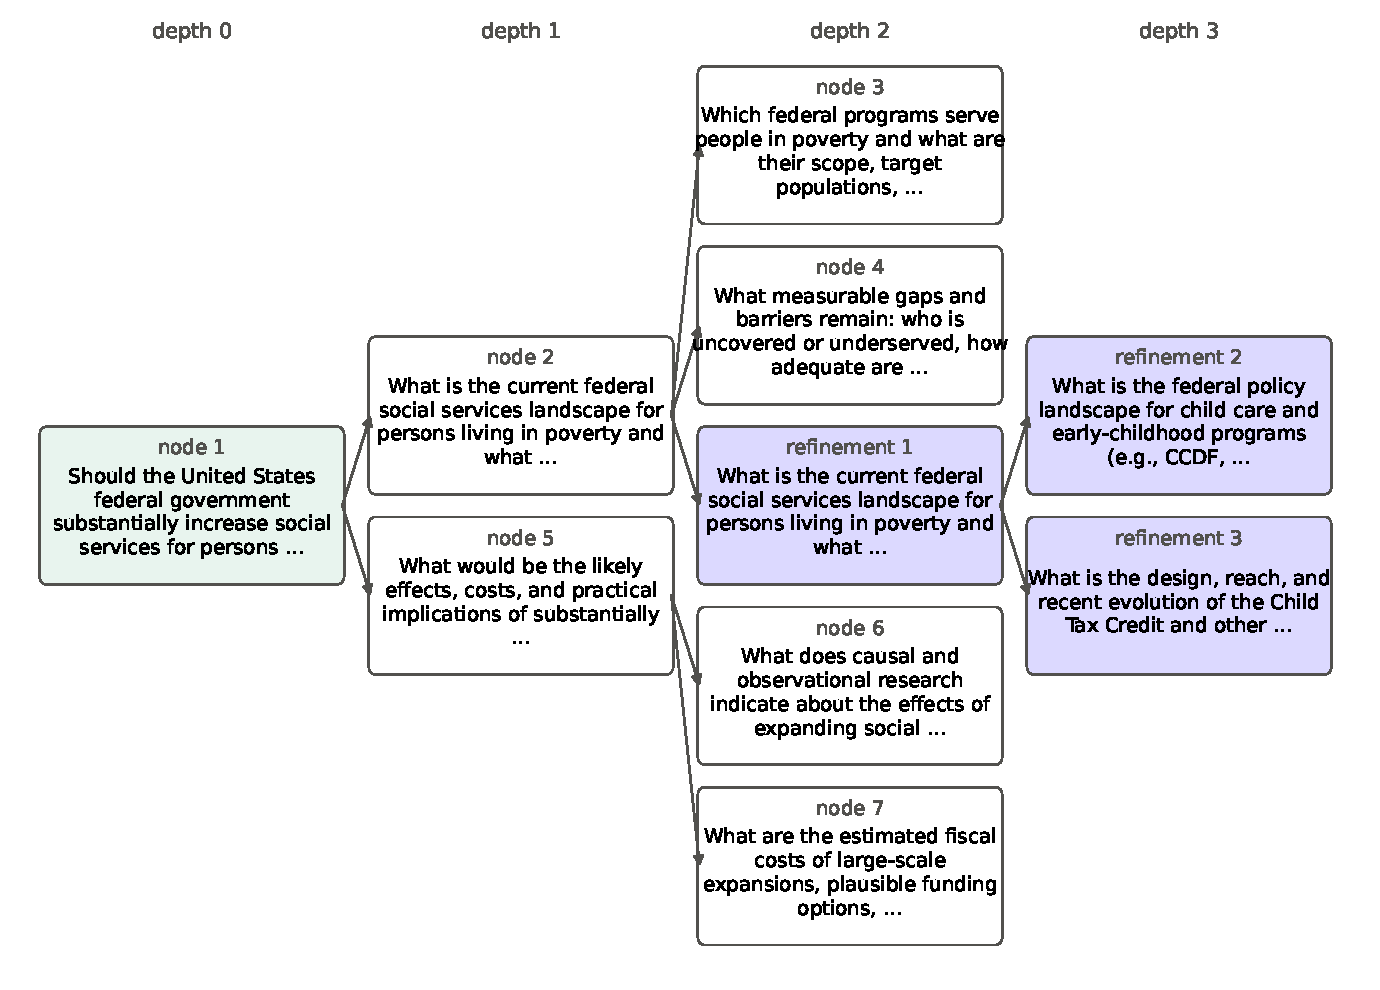
\includegraphics[width=\linewidth]{figs/example_dag.pdf}
\caption{A generated and refined DAG. Arrows indicate parent $\rightarrow$ child. Nodes shaded were added when the refinement step found the composed answer for node 2 to be incomplete.}
\label{fig:dag}
\end{figure}

\section{Code Versions}
\label{app:changes}
There are three versions of the pipeline relevant to this study, two of which we have available.
\begin{enumerate}
    \item \textbf{Evaluated version.} The reports we included in \Cref{sec:experiments,sec:analysis} were finalized on 2 December 2025. The prompts for this version are reproduced in \Cref{app:prompts}, and are the same as those included in our course report. In this version of the pipeline, the DAG is built one layer at a time, composition instructions are written on a second pass, gaps are identified by a two-pass explorer and evaluator, and the bibliography separates cited and uncited sources. We do not include the code for this version in the public repository.
    \item \textbf{Repository version.} This is the state of the code as of the last commit in the repository (26 November 2025), which generates the entire DAG and its composition directions in a single call (\texttt{FullDAGGenerationSignature}). In this version a single validator (\texttt{CompositionValidator}) is used to check for gaps, and it reports none unless a core aspect of the question is missing. The logged run in \Cref{app:dag} was performed with this version, and the citation processing in this version is what we analyze in \Cref{sec:mechanism}. The course report mentions that citations were given global numbers later on, but this does not appear to have been done in this version.
    \item \textbf{Corrected version.} This is the state of the code in the public repository, which is the repository version made configurable for the model provider, with unused code removed, and with the correction described in \Cref{sec:citations}. This correction consists of 5 steps: assigning global numbers to citations, replacing node references with source citations, revising prompts, adding an attribution audit (\texttt{utils/citations.py}, \texttt{utils/attribution\_audit.py}), and including tests to replay the logged run.
\end{enumerate}
% CHECK with Justin: is the evaluated version (Gradescope submission) available? If so, add it to the repository and confirm whether its parent composition still passed leaf-local citation numbers.

\section{Report Statistics by Motion}
\label{app:reports}
\Cref{tab:reports} shows the word count and number of unique sources cited in the body of each report retained in the analysis. The medians in \Cref{tab:text} are based on these metrics.

\begin{table}[t]
\centering
\small
\begin{tabular}{p{6.4cm}rrrrr}
\toprule
Motion & \multicolumn{3}{c}{\sys{}} & \multicolumn{2}{c}{STORM} \\
\cmidrule(lr){2-4}\cmidrule(lr){5-6}
 & words & cited & listed & words & cited \\
\midrule
Human creativity will not remain fundamentally irreducible to artificial intelligence when\,\ldots & 1{,}235 & 8 & 31 & 1{,}991 & 32 \\
Individuals have a moral duty to prioritize the well-being of strangers equally to the\,\ldots & 1{,}523 & 8 & 38 & 1{,}887 & 22 \\
Investing in companies developing foundation models -e.g., OpenAI, Anthropic- will yield\,\ldots & 1{,}247 & 9 & 37 & 2{,}712 & 30 \\
Israel and Palestine should pursue a long-term joint economic zone to promote regional\,\ldots & 1{,}363 & 9 & 35 & 3{,}763 & 35 \\
It is ethically justified for hedge funds to use alternative data sources (e.g., satellite\,\ldots & 1{,}594 & 10 & 30 & 2{,}797 & 24 \\
Moral systems rooted in theism are preferable to non-theistic moral systems. & 1{,}393 & 11 & 36 & 2{,}010 & 23 \\
The benefits of the African Continental Free Trade Area outweigh the harms & 1{,}195 & 7 & 38 & 2{,}376 & 32 \\
The U.S. Federal Reserve should prioritize maintaining high interest rates over stimulating\,\ldots & 1{,}226 & 7 & 32 & 3{,}265 & 24 \\
The U.S. should develop wind, solar, and geothermal energy projects in the Arctic to\,\ldots & 1{,}315 & 13 & 33 & 2{,}477 & 32 \\
U.S. semiconductor manufacturers will outperform global peers over the next decade due to\,\ldots & 1{,}605 & 8 & 39 & 2{,}014 & 23 \\
\bottomrule
\end{tabular}

\caption{Word count and number of unique sources cited in the body of each report retained in the analysis. For \sys{} we also include the number of sources listed in the bibliography.}
\label{tab:reports}
\end{table}

\section{Stance Labels}
\label{app:stance}
Stance labels in \Cref{tab:stance} are assigned by reading the title and final paragraph of each \sys{} report. We store each label and a short quote of the final paragraph of each report in the repository (\texttt{data/reports/stance\_labels.json}), so that all labels can be verified against the report text.
% CHECK with Jessie and Justin: read the ten final paragraphs and confirm the labels.

\section{Word Lists}
\label{app:lexicon}
Rates in \Cref{tab:text} are based on whole-word, case-insensitive counts per 1{,}000 body words. The word lists are organized according to the categories in \citet{hyland2005metadiscourse} as they apply to argumentative reports.
\begin{description}
\item[Hedges.] may, might, could, possibly, perhaps, arguably, potentially, appears, appear, seems, seem, suggests, suggest, likely, unlikely, uncertain, unclear, debated, contested, controversial, depends, depending, can be, to some extent, in some cases, remains open.
\item[Contrast markers.] however, on the other hand, conversely, while, whereas, although, though, nevertheless, nonetheless, critics, opponents, proponents, detractors, both sides.
\item[Commitment markers.] must, should, clearly, demonstrates, demonstrate, shows, show, proves, establishes, therefore, thus, decisively, undeniably, strongly, essential, necessary, outweigh, outweighs, superior, preferable.
\item[Causal connectives.] because, therefore, thus, hence, as a result, consequently, leads to, lead to, led to, results in, result in, resulting in, drives, drive, causes, cause, due to, which means, so that, enables, enable, reduces, increases, raises, lowers.
\end{description}
